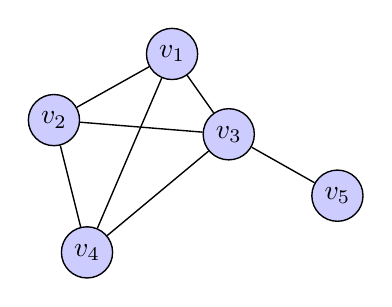
\begin{tikzpicture}[
  scale=0.6,
  vnode/.style={circle, fill=blue!20, draw=black, line width=0.5pt, inner sep=2pt, minimum size=6.5mm},
  edge/.style={line width=0.5pt, draw=black}
]

  % Posicionamiento de vértices asimétrico
  \node[vnode] (v1) at (0, 3.2) {$v_1$};
  \node[vnode] (v2) at (-2.5, 1.8) {$v_2$};
  \node[vnode] (v3) at (1.2, 1.5) {$v_3$};
  \node[vnode] (v4) at (-1.8, -1.0) {$v_4$};
  \node[vnode] (v5) at (3.5, 0.2) {$v_5$};

  % Aristas
  \draw[edge] (v1) -- (v2);
  \draw[edge] (v1) -- (v3);
  \draw[edge] (v2) -- (v4);
  \draw[edge] (v3) -- (v4);
  \draw[edge] (v3) -- (v5);
  \draw[edge] (v2) -- (v3);
  \draw[edge] (v1) -- (v4);

\end{tikzpicture}
